\section{Multi-dimensional inner product relation module}\label{sec:mdipr}

\begin{wrapfigure}{r}{0.5\textwidth}
    \centering
    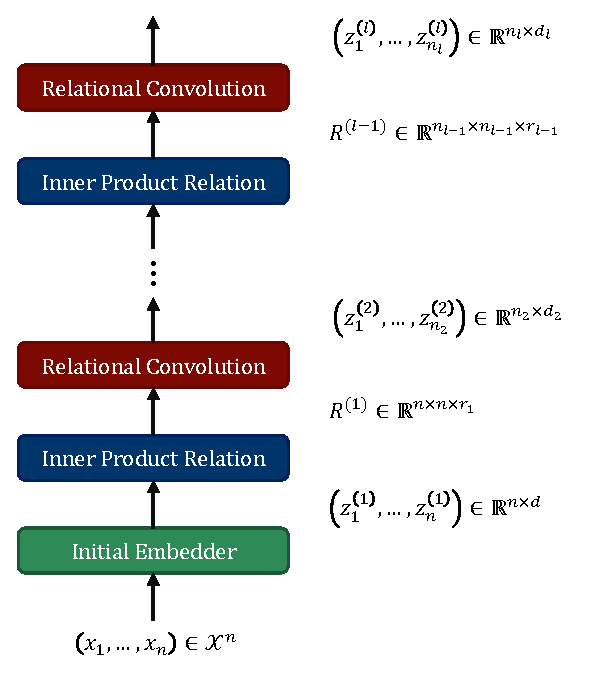
\includegraphics[width=.48\textwidth]{figs/relconv_architecture.pdf}
    % \vskip-12pt
    \caption{Proposed architecture for relational convolutional networks. Hierarchical relations are modeled by iteratively computing pairwise relations between objects and convolving the resultant relation tensor with graphlet filters representing templates of relations between groups of objects.
    }\label{fig:relconv_architecture}
    % \vskip-12pt
\end{wrapfigure}

A relation function is a function that maps a pair of objects $x, y \in \calX$ to a vector representing the relations between the two objects. For example, a relation may represent the information ``$x$ has the same color as $y$, $x$ is larger than $y$, and $x$ is to the left of $y$''. In principle, this can be modeled by an arbitrary learnable function on the concatenation of the two objects' feature representations. For example,~\citet{santoroSimpleNeural2017} models relations by MLPs applied to the concatenation of pairs of objects. However, this approach is missing some crucial inductive biases. In particular, there is no constraint that the learned pairwise function is in fact \textit{relational}---it may just as well represent non-relational object-level information (e.g., ``$x$ is bright and $y$ is small'').%, as opposed to relational information like ``$x$ is larger than $y$''.

% Recent work on relational representation learning has explored using \textit{inner products} to model relations between objects~\citep[e.g.,][]{webbEmergentSymbols2021, kergNeuralArchitecture2022, altabaaAbstractorsRelationalCrossattention2024}. 
Following previous work~\citep[e.g.,][]{webbEmergentSymbols2021, kergNeuralArchitecture2022, altabaaAbstractorsRelationalCrossattention2024}, we propose modeling pairwise relations between objects via \textit{inner products} of feature maps.
The advantage of this approach is that it provides added pressure to learn explicitly relational representations, disentangling relational information from attributes of individual objects, and inducing a geometry on the object space $\calX$.
%  which allows objects to be described in relation to each other. 
For example, in the symmetric case, the inner product relation $r(x,y) = \iprod{\phi(x)}{\phi(y)}$ satisfies symmetry, positive definiteness, and induces a pseudometric on $\calX$. The triangle inequality of the pseudometric expresses a transitivity property---if $x$ is related to $y$ and $y$ is related to $z$, then $x$ must be related to $z$.

More generally, we can allow for multi-dimensional relations by having multiple encoding functions, each extracting a feature to compute a relation on. Furthermore, we can allow for asymmetric relations by having different encoding functions for each object. Hence, we model relations by
\begin{equation}\label{eq:relation_function}
    r(x, y) = \paren{
        \iprod{\phi_1(x)}{\psi_1(y)},\, \ldots,\, \iprod{\phi_{d_r}(x)}{\psi_{d_r}(y)}},
\end{equation}
where $\phi_1, \psi_1, \ldots, \phi_{d_r}, \psi_{d_r}$ are learnable functions. 
% For each dimension of the relation function, the maps $\phi_k, \psi_k$ extract a particular attribute of the objects which is then compared by the inner product. 
The intuition is that, for each dimension, the encoders extract, or `filter' out, particular attributes of the objects and the inner products compute similarity across each attribute.
% A relation, in this sense, is similarity across a particular attribute. 
In the asymmetric case, the attributes extracted from the two objects are different, resulting in an asymmetric relation where a particular attribute of the first object is compared with a different attribute of the second object. For example, this can model relations of the form ``$x$ is brighter than $y$'' (an antisymmetric relation).

\citep{altabaaApproximationRelationFunctions2024} analyzes the function approximation properties of neural relation functions of the form of~\Cref{eq:relation_function}. In particular, they characterize the function class of inner products of neural networks in both the symmetric case and the asymmetric case. They show that in the symmetric case (i.e., $\phi = \psi$), inner products of MLPs are universal approximators for symmetric positive definite kernels. In the asymmetric case, they show that inner products of MLPs are universal approximators for continuous bivariate functions. The efficiency of approximation is characterized in terms of a bound on the number of neurons needed to achieve a particular approximation error.

To promote weight sharing, we can have one common non-linear map $\phi$ shared across all dimensions together with different linear projections for each dimension of the relation. That is, $r: \calX \times \calX \to \reals^{d_r}$ is given by
% \begin{equation}\label{eq:relation_function_lin_proj}
%     r(x, y) = \paren{\iprod{W_1^{(1)}\phi(x)}{W_2^{(1)}\phi(y)},\, \ldots,\, \iprod{W_1^{(d_r)}\phi(x)}{W_2^{(d_r)}\phi(y)}},
% \end{equation}
\begin{equation}\label{eq:relation_function_lin_proj}
    r(x, y) = \paren{\iprod{W_1^{k}\phi(x)}{W_2^{k}\phi(y)}}_{k \in [d_r]},
\end{equation}
where the learnable parameters are $\phi$ and $W_1^{k}, W_2^{k}, k \in [d_r]$. The non-linear map $\phi: \calX \to \reals^{d_\phi}$ may be an MLP, for example, and $W_1^{k}, W_2^{k}$ are $d_{\mathrm{proj}} \times d_\phi$ matrices. The class of functions realizable by~\cref{eq:relation_function_lin_proj} is the same as~\cref{eq:relation_function} but enables greater weight sharing.

The ``Multi-dimensional Inner Product Relation'' (MD-IPR) module receives a sequence of objects $(x_1, \ldots, x_n)$ as input and models the pairwise relations between them by~\cref{eq:relation_function_lin_proj}, returning an $n \times n \times d_r$ relation tensor, $R[i,j] = r(x_i, x_j)$, describing the relations between each pair of objects.
